\documentclass[a4paper,oneside]{article}
%\usepackage[frenchb]{babel}
\usepackage[utf8]{inputenc}
\usepackage[T1]{fontenc}
\usepackage{graphicx}
\usepackage{amssymb}
\usepackage{amsmath}
\usepackage[colorlinks,linkcolor=blue]{hyperref}
\usepackage{fullpage}
\usepackage{titlesec}
\usepackage{fancyhdr}
\usepackage{nopageno}
%%%%%%%%%%%%%%%%%%%%%%%%%
\title{Rapport du Projet de Fin d'Année}
\author{}
\date{}
\makeatletter
\pagestyle{fancy}
\fancyhf{}
\fancyhead[L]{}
\fancyhead[C]{}
\fancyhead[R]{}
\renewcommand{\headrulewidth}{0pt}
\fancyfoot[L]{\@title}
\fancyfoot[C]{}
\fancyfoot[R]{page \thepage / \pageref{myLastPage}}
\renewcommand{\footrulewidth}{0.4pt}
%%%%%%%%%%%%%%%%%%%%%%%%%
\begin{document}
%%%%%%%%%%%%%%%%%%%%%%%%%
\thispagestyle{empty}
\Large
ULCO - L3 Informatique
\vfill
\Huge
\begin{center}
\@title
\end{center}
\normalsize
\vfill
\paragraph{Étudiants : Eric SAILLY, Baptiste FAMCHON, Kossi EHO}
\paragraph{Encadrant : Julien DEHOS }
\paragraph{Date de début : 06 Juin 2016}
\paragraph{Date de fin : 24 Juin 2016 }
\paragraph{Objet du projet : Projet de Fin d'Etude}
~
\vfill
\noindent\rule{\linewidth}{0.5pt}
\tableofcontents
~\\
\noindent\rule{\linewidth}{0.5pt}
\clearpage
%%%%%%%%%%%%%%%%%%%%%%%%%
\section{Présentation du projet}
\subsection{Contexte}


 
Dans le cadre du projet de fin de Licence, il nous était demandé de choisir entre :


	- Le développement d'une plate-forme Web pour le jeu de cartes Pokémon


	- La réalisation d'un jeu en réseau sous C++

Les deux projets nous intéressaient ; l'un proposait une gestion de projet attractive dans un groupe de 8, il permettait de découvrir de nouveaux langages et concepts ( Node JS, Jade, Javascript).

 Ayant appris le C++ au cours du semestre, le deuxième projet nous permettait d'approfondir certaines notions comme la programmation événementielle, la gestion réseau en C++, celle d'un projet en petit groupe ( 3/4 personnes ).
C'est pour ces raisons que nous l'avons choisi ! Il fallait alors se fixer sur un jeu à réaliser, l'idée de la bataille navale est venue grâce à l'ancien travail du collègue…
\subsection{Besoins, spécifications des demandes}


Pour le projet, il nous était demandé de réaliser un jeu en réseau avec une interface graphique. Le langage C++ était imposé, ainsi que l'utilisation de l'API SFML.
Pour créer le logiciel, aucun templates n'était fourni. Il a été écrit par l'équipe de la première à la dernière ligne de code...
Au niveau des spécifications, nous nous sommes donc basés sur celles du jeu en lui même en y ajoutant nos règles :


	- Un plateau de 10*10 cases


	- 2 joueurs, au tour à tour


	- Une flotte composée d'un porte avion ( 5 cases ), un croiseur ( 4 cases ), 2 sous-marins ( 3 cases ), un torpilleur ( 2 cases ), une annexe ( 1 case )


	- Le placement des bateaux se fait en horizontale et/ou verticale


	- Il est possible de coller les bateaux, mais impossible de les croiser


	- Le gagnant est celui qui coule en premier la flotte de l'adversaire. En cas de déconnexion, l'autre joueur devient gagnant. 
	Les joueurs sont informés du résultat grâce à une pop-up.

	- Les joueurs peuvent consulter les règles de jeu


	- Jouer en réseau sur deux ordinateurs différents


	- Le serveur se lance manuellement


	- À travers un menu, ils peuvent rejoindre une partie et saisir un pseudo


	- Positionner leur flotte manuellement ou aléatoirement sur l'écran d'attente


	- Valider cette flotte et passer en attente du deuxième joueur


	- Le jeu se lance quand deux joueurs sont prêts


	- En jeu, chaque joueur dispose de sa flotte et de ses coups tentés


	- Les informations apparaissent en haut de l'écran :

		- Joueur courant

		- Touché / manqué / coulé


	- L'un après l'autre, ils vont choisir une case à attaquer en cliquant dessus.
	
	
	- Une fois la partie terminée, les joueurs sont redirigés vers le menu.

\clearpage


\section{Réalisation}
\subsection{Présentation du logiciel}

Nous avons réalisé un Makefile personnalisé pour compiler deux programmes. L'un concerne le lancement du jeu côté client, l'autre le lancement du serveur. 
Il est également possible de générer, via la commande "make doc", une documentation de notre code.

Pour utiliser notre logiciel, le client lance un serveur manuellement en console, en spécifiant, si besoin, le port souhaité. Nous l'avons placé en 5500 par défaut.
 \\
 \begin{center}
 	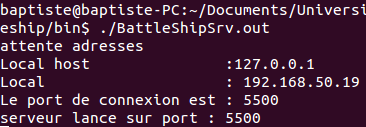
\includegraphics[width = 0.7\linewidth, height = 0.1\textheight ]{serveur.png}
 \end{center}
 
 
Il lance ensuite le jeu avec le programme client. 


Le menu apparait, il pourra alors: 


	- Consulter les règles du jeu


	- Se connecter à un serveur avec une adresse IP


	- Quitter le logiciel grâce aux boutons correspondants


Pour répondre à la demande du client en cours de projet, nous avons implémenté la saisie manuelle d'un port sur le menu...
\\
\begin{center}
	
	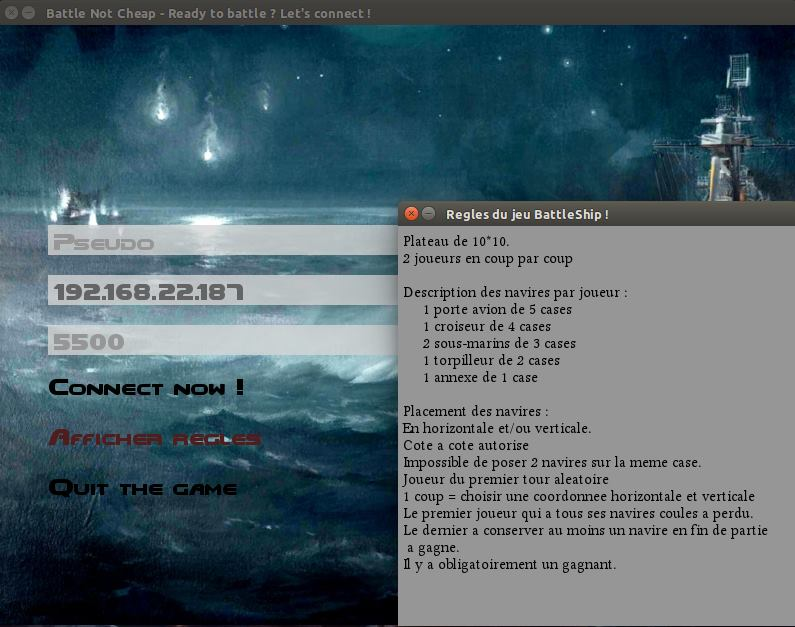
\includegraphics[width = 0.6\linewidth, height = 0.3\textheight ]{Ecran_de_connexion.jpg}
\end{center}


Si le pseudo choisit est déjà pris par l'autre joueur, un message d'erreur s'affiche:
\\
\begin{center}
	
	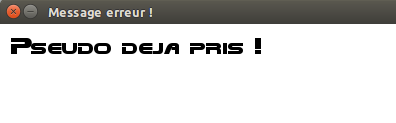
\includegraphics[width = 0.8\linewidth, height = 0.2\textheight ]{pseudoerror.png}
	\end{center}


Une fois connecté au serveur, le joueur choisit la position de sa flotte. Il peut la positionner aléatoirement avec le bouton, ou manuellement:


	- Un double clic tourne le bateau


	- Un drag and drop permet de les positionner
	

Une liste des joueurs connectés est affichée:


	- NotInit signifie qu'il manque un joueur


	- Le pseudo de l'autre personne s'affiche sinon


Si le joueur a terminé son placement, il clique sur le radis et passe à l'écran de jeu.
\\
\begin{center}
 	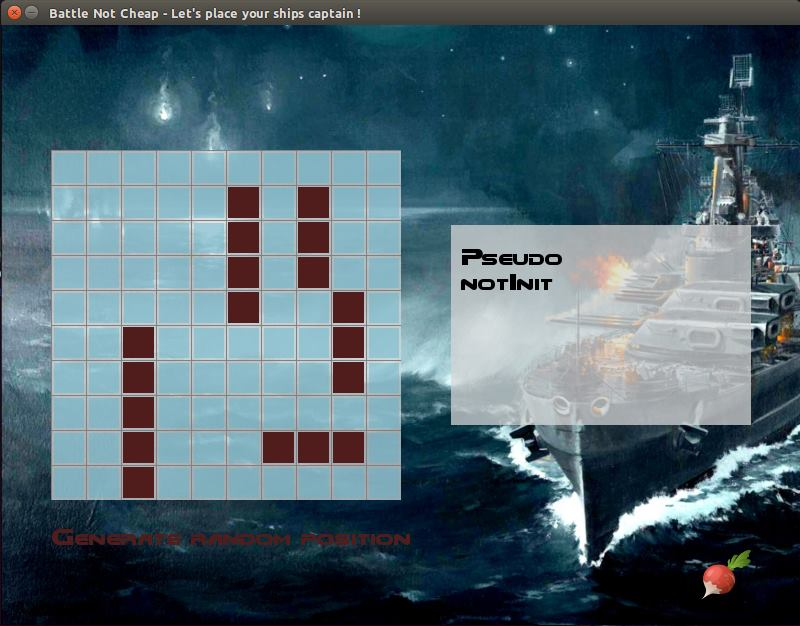
\includegraphics[width = 0.6\linewidth, height = 0.3\textheight ]{Ecran_attente.jpg}
\end{center}
 
Le jeu démarre une fois que les deux joueurs sont prêts. Chacun dispose d'un affichage de sa flotte et de ses coups tentés chez l'adversaire:
\\ 
\begin{center}
	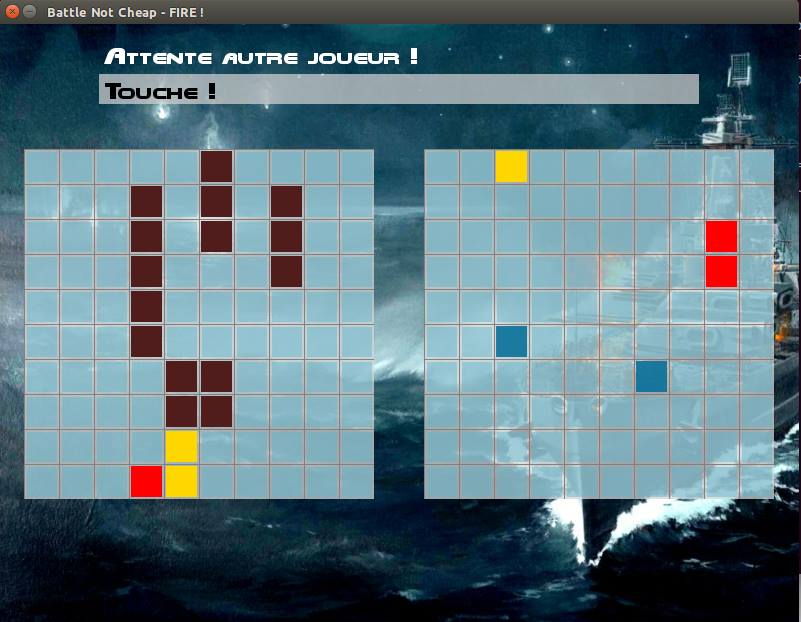
\includegraphics[width = 0.6\linewidth, height = 0.3\textheight ]{Ecran_de_jeu.jpg}
\end{center}


Les informations relatives à l'évolution de la partie apparaissent en haut de l'écran:


	- Qui doit jouer


	- Coup manqué, touché, ou coulé

\clearpage

Ils choisissent à tour de rôle leur attaque, en cliquant sur la case correspondante.


La partie peut se terminer de deux manières:


	- Un des joueurs n'a plus de bateaux en vie, il perd la partie et une fenêtre s'affiche chez les deux joueurs.


	- Un joueur se déconnecte de la partie, l'autre devient gagnant.

 
Une fois la partie terminée, les joueurs sont redirigés vers le menu.


\subsection{Présentation technique}

Nous avons eu l'occasion, pendant les sécances de TP, d'étudier l'architecture "modèle - vue - contrôleur". 
Elle permet d'avoir un code bien organisé et de mieux se représenter le rôle de chaque classe.
\\
Nous nous en sommes inspiré, en y intégrant la notion de réseau:
\\

\begin{center}
		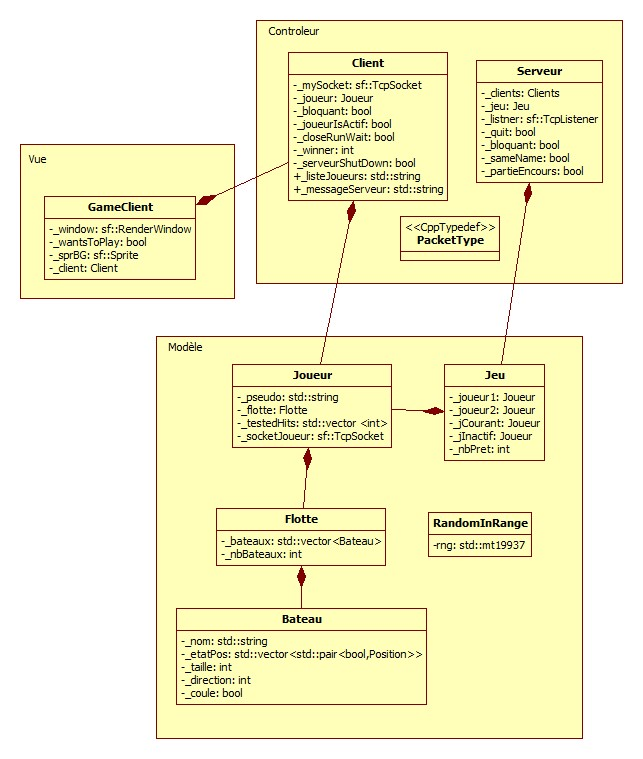
\includegraphics[width = 0.5\linewidth, height = 0.5\textheight ]{MVC_BattleShip.jpg}
\end{center}

\subsection{Gestion du réseau}

Concernant les échanges clients - serveur, nous nous sommes orientés vers le TCP. 
Notre jeu se jouant tour à tour et non en temps réél, l'utilisation de l'UDP ne se justifiait pas. 
\\
Nous avons donc préféré sécuriser les transmissions.
\\
Afin d'éviter la triche, nous avons préféré coder le serveur et le client séparément ;
de ce fait, un joueur ne peut avoir accès aux données de l'autre. 
\clearpage
\subsection{Organisation du code}

Pour l'écriture des classes de la couche modèle, nous avons réalisé régulièrement des tests unitaires.
L'utilisation de la librairie Boost Test nous a permis d'assurer le fonctionnement des méthodes régulièrement appelées.
\\
Concernant la couche vue et contrôleur, nous avons préféré écrire directement de petites foctionnalités et les tester au fur et à mesure. Par exemple:
\\
	- Commencer par tester l'affichage d'un message au clic
\\
	- Afficher ensuite les coordonées du clic dans la grille
\\
	- Tourner le bateau correspondant à ces coordonnées
\\
\clearpage
%%%%%%%%%%%%%%%%%%%%%%%%%

\section{Bilan}

\subsection{Déroulement du projet}


Au choix du jeu, nous avons eu beaucoup d'idées pour le rendre original:

 
	- Mode 4 joueurs, avec adaptation de grilles


	- Pouvoir jouer contre une intelligence artificielle 


	- Débloquer des bonus en fonction de l'avancement


	- Pouvoir jouer sans réseau


	- Développer une interface graphique avec des batailles sous-marines et aériennes... 
\\

Après réflexions, nous nous sommes concentrés sur les points essentiels afin de rendre un logiciel propre et fonctionnel... Quitte à implémenter, plus tard, d'autres fonctionnalités.
\\

La première semaine fut consacrée au brainstorming. Une première difficulté était d'imaginer l'architecture du logiciel, il fallait y intégrer de nouveaux concepts comme le réseau. 
\\
Vouloir positionner la classe Jeu trop haut dans notre architecture était une erreur. Nous pensions qu'elle contrôlait tout. 
On a compris, une fois le réseau dompté, qu'elle ferait parti de la couche "Modèle" plutôt que "Contrôleur". Notre situation s'est alors débloquée. 


Nous avons réalisé des croquis d'échange client - serveur, des morceaux d'UML que l'on venait compléter et modifier, au fur et à mesure des idées.


Le réseau a aussi posé beaucoup de problèmes. L'idée était d'encoder, puis d'envoyer les paquets d'un côté ; les recevoir, puis les décoder de l'autre.

 
Mais comment lier ce principe avec la SFML? 


Pour la réalisation de cette partie, nous nous sommes aidés de tutoriels sur les forums. À partir des informations récoltées, nous avons bâti un programme de chat indépendant. 
Une fois le principe compris, nous l'avons adapté à notre jeu avec des messages clients-serveurs spécifiques.

Github nous a également posé quelques soucis avec les conflits, parfois explicites, parfois non. Il nous supprimait des morceaux de codes. 
Nous avons décidé de travailler sur des zones différentes en faisant régulièrement des git push and pull pour avoir le même contenu, avant chaque modification.


\subsection{Réalisation des objectifs }


Les besoins du client et les objectifs fixés ont été réalisés. 
C'est en parti grâce aux "concepts trop originaux" que l'on a préféré passer rapidement en perspectives pour se recentrer sur la demande.
\\
Le client a ainsi pu nous suggérer d'autres fonctionnalités en cours de projet, comme la connexion à un port saisi manuellement.
\\
A l'avenir, on pourra alors envisager de sauvegarder et charger une partie, jouer contre une IA, et pourquoi pas intégrer un mode multijoueurs.


\subsection{Conclusion pour les projets futurs}

Une stratégie que l'on pourra réutiliser dans nos futurs projets, est de ne pas se lancer directement dans l'écriture du code. 
Le fait de se concentrer sur l'architecture pendant la première semaine, nous a permis de débloquer rapidement beaucoup de situations et d'y voir plus clair.


Cependant, il serait judicieux de mieux évaluer le temps d'apprentissage des nouvelles technologies ( SFML pour notre cas ), et d'en tenir compte pour éviter les déconvenues.
Nous avons aussi découvert de nouveaux outils comme Doxygen pour créer des documentations de codes automatiques ;
à l'avenir, on pourrait en respecter directement la syntaxe pour plus d’efficacité. 



%%%%%%%%%%%%%%%%%%%%%%%%%
\label{myLastPage}
\end{document}
